
\begin{question}
What do you understand by the term catalysis? Name three different metal catalyst and the reaction catalyzed with them.

\end{question}

\begin{solution}
\textbf{Catalysis} means the lowering of the activation energy $E_a$. It is the process of increasing the rate of a chemical reaction by adding a catalyst, which is not consumed in the course of the reaction.
\vspace{-2.5cm}
\begin{center}
 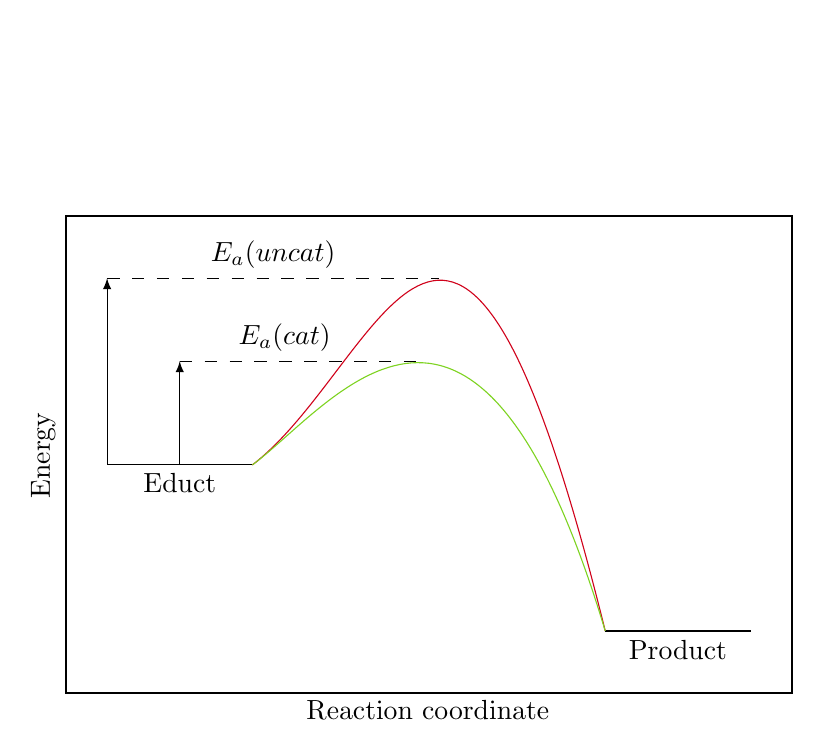
\begin{tikzpicture}[x=0.75pt,y=0.75pt,yscale=-1,xscale=1]
%\path (0,557); %set diagram left start at 0, and has height of 557
%Straight Lines [id:da8963302898593869] 
\draw    (110,130) -- (180,130) ;
%Curve Lines [id:da25528306667553147] 
\draw [color={rgb, 255:red, 208; green, 2; blue, 27 }  ,draw opacity=1 ]   (180,130) .. controls (243.78,80.98) and (278.25,-80.4) .. (350,210) ;
%Straight Lines [id:da9286679635565723] 
\draw    (350,210) -- (420,210) ;
%Curve Lines [id:da5920006668723389] 
\draw [color={rgb, 255:red, 126; green, 211; blue, 33 }  ,draw opacity=1 ]   (180,130) .. controls (220,100) and (287.55,2.25) .. (350,210) ;
%Shape: Rectangle [id:dp9170110896395716] 
\draw  [line width=0.75]  (90,10) -- (440,10) -- (440,240) -- (90,240) -- cycle ;
%Straight Lines [id:da29019500832361755] 
\draw  [dash pattern={on 4.5pt off 4.5pt}]  (110,40) -- (270,40) ;
%Straight Lines [id:da3043530571809191] 
\draw  [dash pattern={on 4.5pt off 4.5pt}]  (145,80) -- (260,80) ;
%Straight Lines [id:da6765322257918037] 
\draw [latex-]   (145,80) -- (145,130) ;
%Straight Lines [id:da6158891760080316] 
\draw [latex-]   (110,40) -- (110,130) ;

% Text Node
\draw (264.5,242) node [anchor=north] [inner sep=0.75pt]   [align=left] {Reaction coordinate};
% Text Node
\draw (72,125.5) node [anchor=north] [inner sep=0.75pt]  [rotate=-270] [align=left] {Energy};
% Text Node
\draw (195.5,76.6) node [anchor=south] [inner sep=0.75pt]    {$E_{a}( cat)$};
% Text Node
\draw (190,36.6) node [anchor=south] [inner sep=0.75pt]    {$E_{a}( uncat)$};
% Text Node
\draw (385,213) node [anchor=north] [inner sep=0.75pt]   [align=left] {Product};
% Text Node
\draw (145,133) node [anchor=north] [inner sep=0.75pt]   [align=left] {Educt};
\end{tikzpicture}

\end{center}
%%
The synthesis of methane:
%%
\begin{equation}
 \ch{CO + 3 H2 ->[Ni] CH4 + H2O}
\end{equation}
%%
The synthesis of methanol:
%%
\begin{equation}
 \ch{CO + 2 H2 ->[Zn,\;Cu-oxide] CH3OH}
\end{equation}
%%
Fischer-Tropsch synthesis:
%%
\begin{equation}
 \ch{$n$ CO + $(2n+1)$ H2 ->[Fe] C_{$n$}H_{$2n+2$} + $n$ H2O}
\end{equation}
\end{solution}
